% Options for packages loaded elsewhere
\PassOptionsToPackage{unicode}{hyperref}
\PassOptionsToPackage{hyphens}{url}
%
\documentclass[
  ignorenonframetext,
]{beamer}
\usepackage{pgfpages}
\setbeamertemplate{caption}[numbered]
\setbeamertemplate{caption label separator}{: }
\setbeamercolor{caption name}{fg=normal text.fg}
\beamertemplatenavigationsymbolsempty
% Prevent slide breaks in the middle of a paragraph
\widowpenalties 1 10000
\raggedbottom
\setbeamertemplate{part page}{
  \centering
  \begin{beamercolorbox}[sep=16pt,center]{part title}
    \usebeamerfont{part title}\insertpart\par
  \end{beamercolorbox}
}
\setbeamertemplate{section page}{
  \centering
  \begin{beamercolorbox}[sep=12pt,center]{part title}
    \usebeamerfont{section title}\insertsection\par
  \end{beamercolorbox}
}
\setbeamertemplate{subsection page}{
  \centering
  \begin{beamercolorbox}[sep=8pt,center]{part title}
    \usebeamerfont{subsection title}\insertsubsection\par
  \end{beamercolorbox}
}
\AtBeginPart{
  \frame{\partpage}
}
\AtBeginSection{
  \ifbibliography
  \else
    \frame{\sectionpage}
  \fi
}
\AtBeginSubsection{
  \frame{\subsectionpage}
}
\usepackage{amsmath,amssymb}
\usepackage{lmodern}
\usepackage{ifxetex,ifluatex}
\ifnum 0\ifxetex 1\fi\ifluatex 1\fi=0 % if pdftex
  \usepackage[T1]{fontenc}
  \usepackage[utf8]{inputenc}
  \usepackage{textcomp} % provide euro and other symbols
\else % if luatex or xetex
  \usepackage{unicode-math}
  \defaultfontfeatures{Scale=MatchLowercase}
  \defaultfontfeatures[\rmfamily]{Ligatures=TeX,Scale=1}
\fi
\usecolortheme{dolphin}
% Use upquote if available, for straight quotes in verbatim environments
\IfFileExists{upquote.sty}{\usepackage{upquote}}{}
\IfFileExists{microtype.sty}{% use microtype if available
  \usepackage[]{microtype}
  \UseMicrotypeSet[protrusion]{basicmath} % disable protrusion for tt fonts
}{}
\makeatletter
\@ifundefined{KOMAClassName}{% if non-KOMA class
  \IfFileExists{parskip.sty}{%
    \usepackage{parskip}
  }{% else
    \setlength{\parindent}{0pt}
    \setlength{\parskip}{6pt plus 2pt minus 1pt}}
}{% if KOMA class
  \KOMAoptions{parskip=half}}
\makeatother
\usepackage{xcolor}
\IfFileExists{xurl.sty}{\usepackage{xurl}}{} % add URL line breaks if available
\IfFileExists{bookmark.sty}{\usepackage{bookmark}}{\usepackage{hyperref}}
\hypersetup{
  pdftitle={Präsentation - Gruppe 1},
  pdfauthor={Annika Janson; Jan Beck},
  hidelinks,
  pdfcreator={LaTeX via pandoc}}
\urlstyle{same} % disable monospaced font for URLs
\newif\ifbibliography
\usepackage{longtable,booktabs,array}
\usepackage{calc} % for calculating minipage widths
\usepackage{caption}
% Make caption package work with longtable
\makeatletter
\def\fnum@table{\tablename~\thetable}
\makeatother
\usepackage{graphicx}
\makeatletter
\def\maxwidth{\ifdim\Gin@nat@width>\linewidth\linewidth\else\Gin@nat@width\fi}
\def\maxheight{\ifdim\Gin@nat@height>\textheight\textheight\else\Gin@nat@height\fi}
\makeatother
% Scale images if necessary, so that they will not overflow the page
% margins by default, and it is still possible to overwrite the defaults
% using explicit options in \includegraphics[width, height, ...]{}
\setkeys{Gin}{width=\maxwidth,height=\maxheight,keepaspectratio}
% Set default figure placement to htbp
\makeatletter
\def\fps@figure{htbp}
\makeatother
\setlength{\emergencystretch}{3em} % prevent overfull lines
\providecommand{\tightlist}{%
  \setlength{\itemsep}{0pt}\setlength{\parskip}{0pt}}
\setcounter{secnumdepth}{-\maxdimen} % remove section numbering
\ifluatex
  \usepackage{selnolig}  % disable illegal ligatures
\fi

\title{Präsentation - Gruppe 1}
\subtitle{Factors that impact {[}Jan's{]} study performance}
\author{Annika Janson \and Jan Beck}
\date{9.6.2021}

\begin{document}
\frame{\titlepage}

\begin{frame}{Einführung}
\protect\hypertarget{einfuxfchrung}{}
\begin{block}{Ausgangsdaten}
\protect\hypertarget{ausgangsdaten}{}
\begin{itemize}
\tightlist
\item
  Jan studiert seit WS 2018 BaWiso an der WU
\item
  Sekundengenaue Zeiterfassungsdaten von 27.8.2018-28.5.2021
\item
  Kategorisiert nach LV und Art der Lernaktivität (z.B.
  ``Gruppenarbeit'', ``Prüfungsvorbereitung'')
\item
  1153 Observationen
\end{itemize}

\begin{figure}
\centering
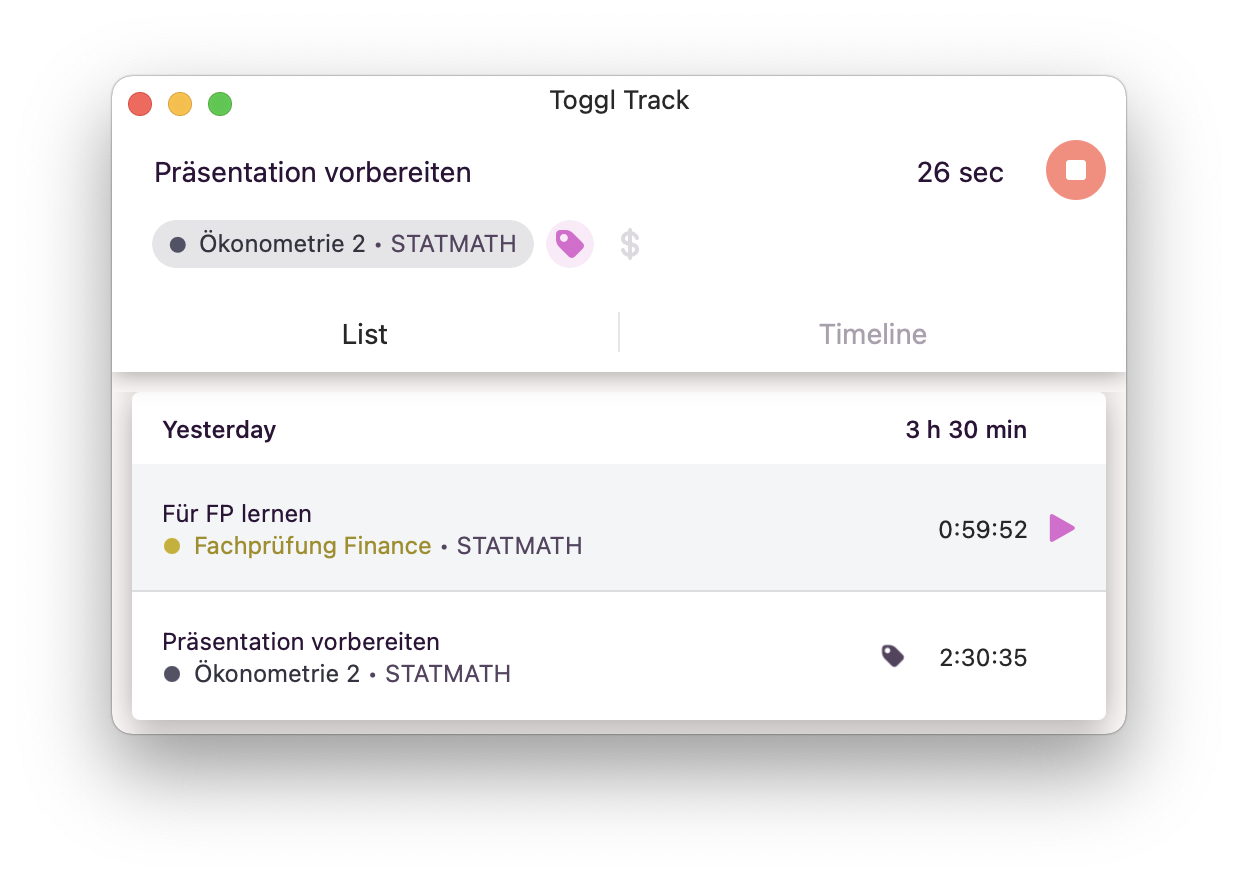
\includegraphics{images/toggl.png}
\caption{Zeiterfassung}
\end{figure}
\end{block}
\end{frame}

\begin{frame}
\begin{block}{Forschungsfrage}
\protect\hypertarget{forschungsfrage}{}
\begin{itemize}
\item
  Lässt sich die Lernleistung erklären/vorhersagen?

  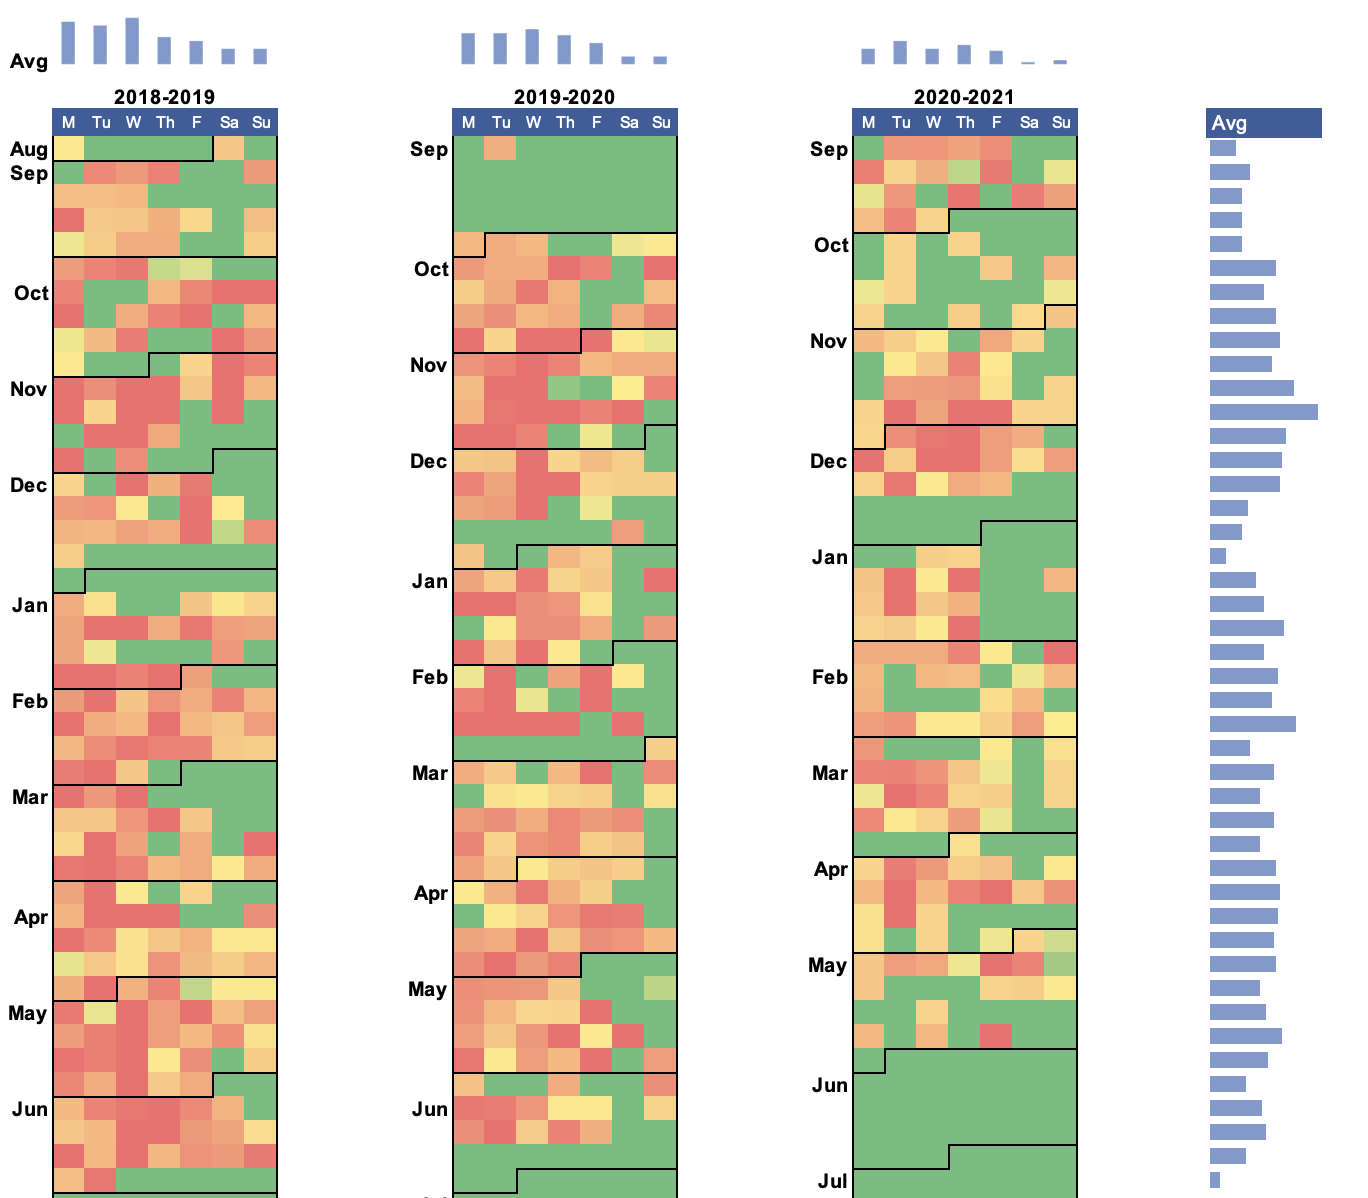
\includegraphics{images/heatmap-02.png}
\end{itemize}
\end{block}
\end{frame}

\begin{frame}
\begin{block}{Summary statistics}
\protect\hypertarget{summary-statistics}{}
\begin{itemize}
\item
  Dauer aller Studienaktivitäten: 2223.54 Stunden
\item
  Mean (pro Woche): 15 Stunden. SD: 11
\item
  Extremwerte: 12h 40m 39s (14.11.2018)
\item
  Gruppiert nach Art der Aktivität:\\
  ~\\

  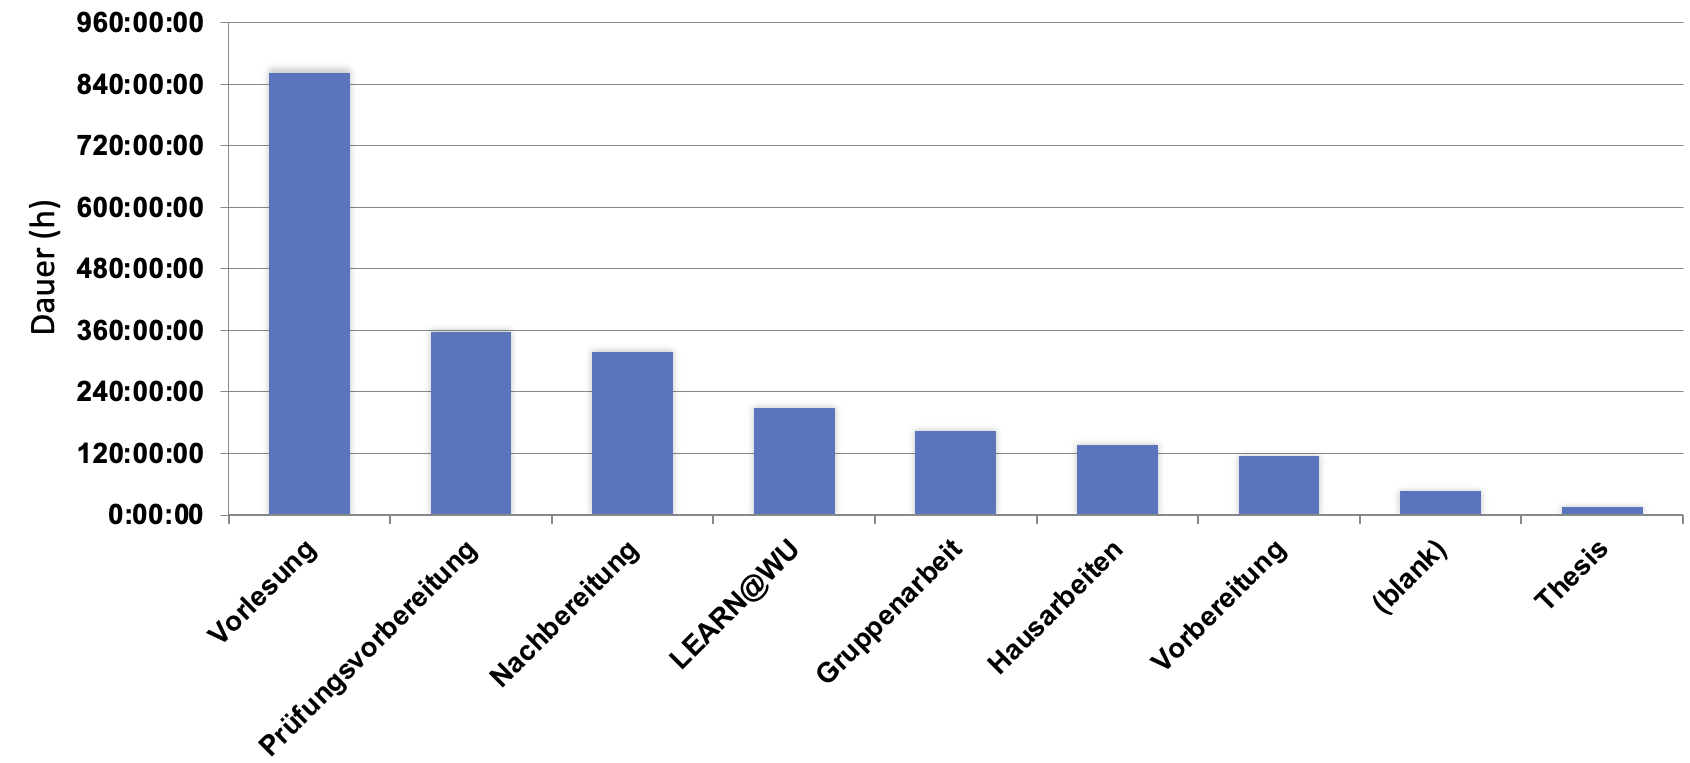
\includegraphics{images/tags.png}
\end{itemize}
\end{block}
\end{frame}

\begin{frame}{Zeitreihenanalyse}
\protect\hypertarget{zeitreihenanalyse}{}
\begin{itemize}
\tightlist
\item
  Abhängige Variable: Wöchentliche Studienaktivität (h)
\item
  Klassisches Regressionsmodel mit Trend
\end{itemize}

\begin{table}[!ht]
\caption{}
\label{} 
\begin{tabular}{ l D{.}{.}{2} } 
\hline 
  & \multicolumn{ 1 }{ c }{ Trend } \\ \hline
 %           & Trend   \\ 
(Intercept) & 19.76 ^*\\ 
            & (1.75)  \\ 
trend       & -0.06 ^*\\ 
            & (0.02)   \\
 $N$         & 144     \\ 
$R^2$       & 0.05    \\ 
adj. $R^2$  & 0.05    \\ 
Resid. sd   & 10.46    \\ \hline
 \multicolumn{2}{l}{\footnotesize{Standard errors in parentheses}}\\
\multicolumn{2}{l}{\footnotesize{$^*$ indicates significance at $p< 0.05 $}} 
\end{tabular} 
 \end{table}
\end{frame}

\begin{frame}
\begin{block}{Einfaches Trendmodel}
\protect\hypertarget{einfaches-trendmodel}{}
\[y_{t}=\mu_{t}+u_{t}\]

\includegraphics{ÖKO2-Presentation_files/figure-beamer/unnamed-chunk-3-1.pdf}
\end{block}
\end{frame}

\begin{frame}
\includegraphics{ÖKO2-Presentation_files/figure-beamer/unnamed-chunk-4-1.pdf}
\end{frame}

\begin{frame}
\begin{block}{Klassisches Regressionsmodel mit Trend und
Season(=Semester)}
\protect\hypertarget{klassisches-regressionsmodel-mit-trend-und-seasonsemester}{}
\begin{longtable}[]{@{}lrrr@{}}
\toprule
& Trend & Trend+Season & Trend*Season \\
\midrule
\endhead
Intercept & 19.7629132 & -3.0142715 & 1.0934288 \\
Trend & -0.0596092 & 0.1355168 & 0.0361113 \\
SS2019 & NA & -10.6384007 & -12.5831787 \\
WS2019 & NA & -23.7967314 & 44.5680048 \\
SS2020 & NA & 0.6923745 & -6.4441159 \\
WS2020 & NA & -4.1715290 & 3.5368673 \\
SS2021 & NA & -19.2564514 & -34.7678981 \\
Trend:SS2019 \%\textgreater\% & NA & 21.4087460 & 21.2758588 \\
Trend:WS2019 & NA & NA & 0.0769066 \\
Trend:SS2020 & NA & NA & -0.4247941 \\
Trend:WS2020 & NA & NA & 0.3245365 \\
Trend:SS2021 & NA & NA & -0.0768198 \\
Aktiv & NA & NA & 0.1966748 \\
\bottomrule
\end{longtable}
\end{block}
\end{frame}

\begin{frame}
\begin{block}{Model mit Trend, Season (=Semester)}
\protect\hypertarget{model-mit-trend-season-semester}{}
\[y_{t}=\mu_{t}+\tilde{s}_{t}+u_{t}\]

\includegraphics{ÖKO2-Presentation_files/figure-beamer/unnamed-chunk-6-1.pdf}
\end{block}
\end{frame}

\begin{frame}
\begin{block}{Model mit Trend, Season (=Semester), Interaktionsterm}
\protect\hypertarget{model-mit-trend-season-semester-interaktionsterm}{}
\[y_{t}=\mu_{t}+\tilde{s}_{t}+\mu_{t}\tilde{s}_{t}+u_{t}\]

\includegraphics{ÖKO2-Presentation_files/figure-beamer/unnamed-chunk-7-1.pdf}
\end{block}
\end{frame}

\begin{frame}
\begin{block}{Residuenanalyse (Model 3)}
\protect\hypertarget{residuenanalyse-model-3}{}
\hfill\break

\includegraphics{ÖKO2-Presentation_files/figure-beamer/unnamed-chunk-8-1.pdf}
\end{block}
\end{frame}

\begin{frame}[fragile]
\begin{longtable}[]{@{}lll@{}}
\caption{Selection criteria of our 3 models}\tabularnewline
\toprule
& AIC & BIC \\
\midrule
\endfirsthead
\toprule
& AIC & BIC \\
\midrule
\endhead
Trend & 1088.874 & 1097.783 \\
Trend+Season & 975.7714 & 1002.5 \\
Trend*Season & 981.1254 & 1022.703 \\
\bottomrule
\end{longtable}

\begin{verbatim}
## 
##  Durbin-Watson test
## 
## data:  seasonal_trend_model2
## DW = 1.9482, p-value = 0.09495
## alternative hypothesis: true autocorrelation is greater than 0
\end{verbatim}
\end{frame}

\begin{frame}{Zeitreihenanalyse}
\protect\hypertarget{zeitreihenanalyse-1}{}
\begin{itemize}
\item
  Abhängige Variable: Wöchentliche Studienaktivität (h)
\item
  Erklärende Variablen:

  \begin{itemize}
  \item
    Wetter: Sonnenstunden (monatlich, Hohe Warte ZAMG)
  \item
    Anzahl Videos auf Youtube geschaut (Google Takeout)
  \item
    Gewicht und Herzschlag, gemessen morgens (bis Anfang 2020)
  \end{itemize}
\end{itemize}

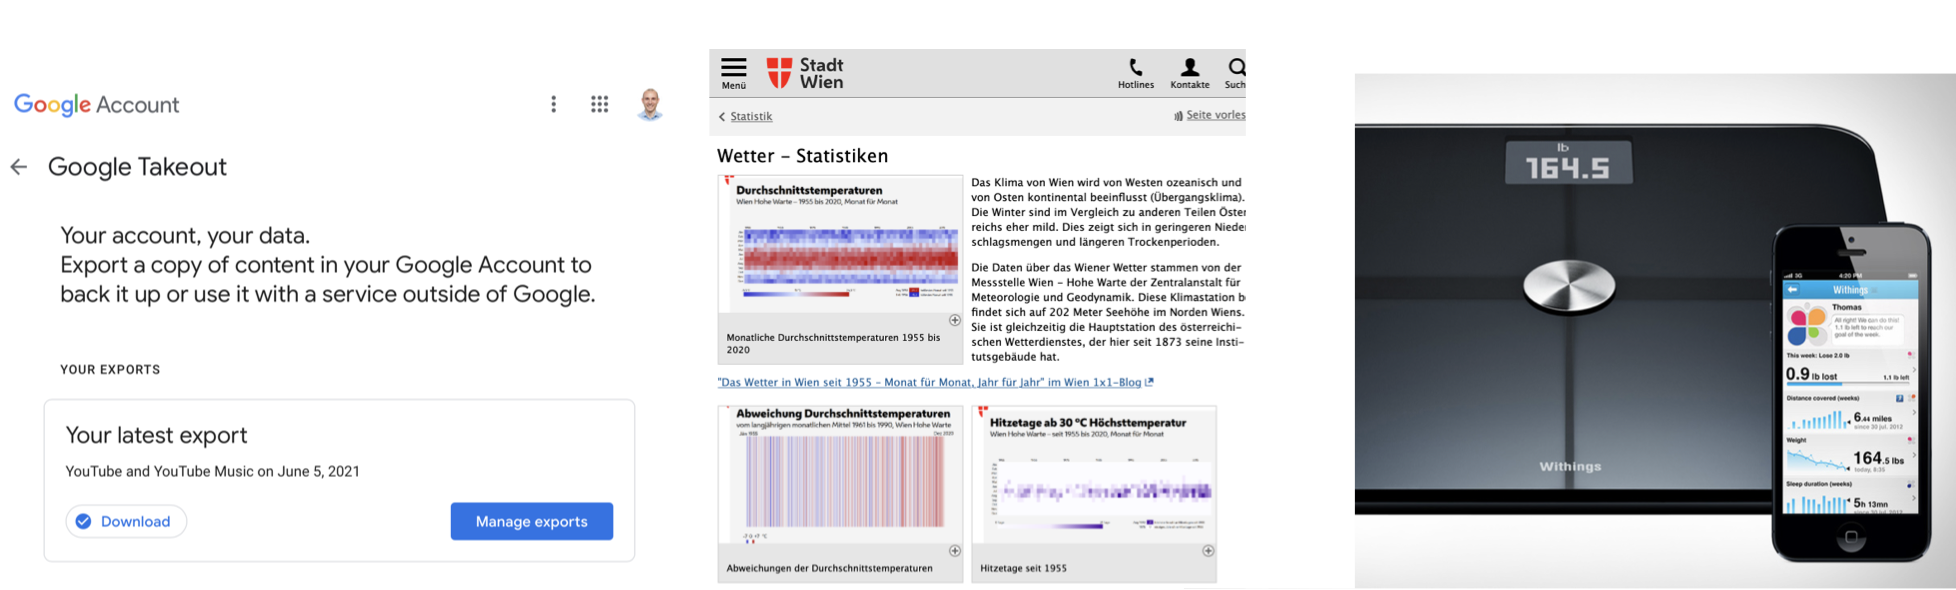
\includegraphics{images/x.png}
\end{frame}

\begin{frame}[fragile]
\begin{block}{Anhang: Externe Variablen}
\protect\hypertarget{anhang-externe-variablen}{}
\begin{verbatim}
##       Sun           Youtube             HP            Weight     
##  Min.   : 7.25   Min.   :  6.00   Min.   :64.67   Min.   :75.30  
##  1st Qu.:18.50   1st Qu.: 61.00   1st Qu.:70.33   1st Qu.:77.09  
##  Median :45.50   Median : 80.00   Median :73.00   Median :78.74  
##  Mean   :41.55   Mean   : 87.29   Mean   :74.32   Mean   :78.73  
##  3rd Qu.:57.00   3rd Qu.:106.00   3rd Qu.:77.53   3rd Qu.:80.55  
##  Max.   :89.00   Max.   :271.00   Max.   :92.00   Max.   :81.83  
##                                   NA's   :92      NA's   :92
\end{verbatim}
\end{block}
\end{frame}

\begin{frame}
\begin{block}{Anhang: Externe Variablen}
\protect\hypertarget{anhang-externe-variablen-1}{}
\includegraphics{ÖKO2-Presentation_files/figure-beamer/unnamed-chunk-11-1.pdf}
\end{block}
\end{frame}

\begin{frame}
\begin{tabular}{ l D{.}{.}{2} } 
\hline 
  & \multicolumn{ 1 }{ c }{ Externes Model } \\ \hline
 %              & Externes Model\\ 
(Intercept)    & 23.37 ^*      \\ 
               & (3.41)        \\ 
Sunny          & -4.82         \\ 
               & (2.58)        \\ 
Youtube        & -0.02         \\ 
               & (0.03)        \\ 
HR.c           & 0.04          \\ 
               & (0.24)        \\ 
Weight.c       & 3.43 ^*       \\ 
               & (0.84)         \\
 $N$            & 52            \\ 
$R^2$          & 0.44          \\ 
adj. $R^2$     & 0.39          \\ 
Resid. sd      & 8.69           \\ \hline
 \multicolumn{2}{l}{\footnotesize{Standard errors in parentheses}}\\
\multicolumn{2}{l}{\footnotesize{$^*$ indicates significance at $p< 0.05 $}} 
\end{tabular}
\end{frame}

\begin{frame}
\begin{block}{Findings}
\protect\hypertarget{findings}{}
\begin{itemize}
\tightlist
\item
  Grundsätzlich abnehmender Trend der Studienleistung
\item
  Semester unterscheiden sich stark im Schnitt und Trend (stärker als
  globaler Trend)
\item
  Wetter, Medienkonsum und Gesundheit erklären mehr Variation in
  Studienaktivität als Trend model
\item
  Jan lernt in sonnigen Monaten im Schnitt c.p. 2.75h weniger (nicht
  signifkant) und sollte vielleicht ein paar Kilo zunehmen
\end{itemize}
\end{block}
\end{frame}

\begin{frame}[fragile]{Probit/Logit model}
\protect\hypertarget{probitlogit-model}{}
\begin{block}{Zusammenhang zwischen Lerndauer/ECTS und Note}
\protect\hypertarget{zusammenhang-zwischen-lerndauerects-und-note}{}
Ordinal logistic regression with multiple categories
\end{block}

\begin{block}{Model 1}
\protect\hypertarget{model-1}{}
Vorhersage der Note bei 4 ECTS:

\begin{verbatim}
##           Value Std. Error   t value    pvalue
## ects 0.07003992  0.6380092 0.1097789 0.9125848
## 1|2  0.45136309  2.5695587 0.1756578 0.8605628
## 2|3  2.06974277  2.5798530 0.8022716 0.4223959
## 3|4  3.08426279  2.6636796 1.1578956 0.2469067
\end{verbatim}

\begin{verbatim}
##          1          2          3          4 
## 0.54269661 0.31417954 0.08602099 0.05710285
\end{verbatim}
\end{block}
\end{frame}

\begin{frame}[fragile]
\begin{block}{Model 2}
\protect\hypertarget{model-2}{}
Vorhersage der Note bei 40h Lernaufwand pro ECTS (also insg. 120h) und 4
ECTS

\begin{verbatim}
##               Value   Std. Error    t value    pvalue
## dauer  0.0006176278 0.0006495865  0.9508015 0.3417051
## ects  -0.0878620635 0.6700858780 -0.1311206 0.8956799
## 1|2    0.3142520079 2.6259968338  0.1196696 0.9047449
## 2|3    2.0132795214 2.6337641289  0.7644115 0.4446221
## 3|4    3.0736324398 2.7151624849  1.1320252 0.2576238
\end{verbatim}

\begin{verbatim}
##          1          2          3          4 
## 0.57325000 0.30693161 0.07479497 0.04502342
\end{verbatim}
\end{block}
\end{frame}

\begin{frame}[fragile]
\begin{block}{Model 3}
\protect\hypertarget{model-3}{}
Vorhersage der Note bei 120h Lernaufwand

\begin{verbatim}
##              Value   Std. Error  t value       pvalue
## dauer 0.0006032514 0.0006312221 0.955688 0.3392298662
## 1|2   0.6535298821 0.6006440834 1.088048 0.2765737060
## 2|3   2.3484122131 0.7700071650 3.049858 0.0022894988
## 3|4   3.4106046700 0.9958406173 3.424850 0.0006151391
\end{verbatim}

\begin{verbatim}
##          1          2          3          4 
## 0.57238266 0.30698560 0.07535611 0.04527563
\end{verbatim}
\end{block}
\end{frame}

\begin{frame}[fragile]
\begin{block}{Korrelationen}
\protect\hypertarget{korrelationen}{}
\begin{verbatim}
## [1] "Korrelation zwischen Dauer und Note: 0.2097"
\end{verbatim}

\begin{verbatim}
## [1] "Korrelation zwichen ECTS und Note: 0.1531"
\end{verbatim}

\begin{verbatim}
## [1] "Korrelation zwischen ECTS und Dauer: 0.2146"
\end{verbatim}
\end{block}
\end{frame}

\begin{frame}
\includegraphics{ÖKO2-Presentation_files/figure-beamer/unnamed-chunk-19-1.pdf}
\end{frame}

\begin{frame}[fragile]
\begin{block}{Korrelation zwischen Youtube und Lernzeit pro Monat}
\protect\hypertarget{korrelation-zwischen-youtube-und-lernzeit-pro-monat}{}
\begin{verbatim}
## [1] 0.5153605
\end{verbatim}

\includegraphics{ÖKO2-Presentation_files/figure-beamer/unnamed-chunk-20-1.pdf}
\end{block}
\end{frame}

\begin{frame}
\begin{block}{Findings}
\protect\hypertarget{findings-1}{}
\begin{itemize}
\tightlist
\item
  Sagt fast immer das Selbe aus, da es fast nur 1er und 2er gibt. Es
  können keine wirklichen Aussagen für sehr hohe oder sehr niedrige
  Stundenzahl an Lernaufwand oder ähnliches vorrausgesagt werden.
\item
  Mit insgesamt 120h Lernaufwand in einem Kurs mit 4 ects schreibt Jan
  mit einer Wahrscheinlichkeit von 57,24\% eine Eins. Aber eine gewisse
  Verzerrung besteht, da die Noten prinzipiell immer eher besser
  ausfallen und der Datensatz nicht ausreichend ist um genaue
  Vorhersagen zu treffen.
\end{itemize}
\end{block}
\end{frame}

\begin{frame}
\begin{block}{Vielen Dank für Ihre Aufmerksamkeit!}
\protect\hypertarget{vielen-dank-fuxfcr-ihre-aufmerksamkeit}{}
\begin{itemize}
\tightlist
\item
  Wir freuen uns auf Ihre Fragen.
\end{itemize}
\end{block}
\end{frame}

\begin{frame}[fragile]
\begin{block}{Anhang Model 3 (Zeitreihenanalyse)}
\protect\hypertarget{anhang-model-3-zeitreihenanalyse}{}
\begin{verbatim}
##                             Estimate Std. Error    t value
## (Intercept)               1.09342881  9.4021936  0.1162951
## trend                     0.03611127  0.2123502  0.1700553
## factor(Semester)2       -12.58317866 19.3040719 -0.6518406
## factor(Semester)3        44.56800483 71.5422043  0.6229610
## factor(Semester)4        -6.44411594  8.7763362 -0.7342604
## factor(Semester)5         3.53686734 15.6287339  0.2263054
## factor(Semester)6       -34.76789815 22.9596987 -1.5143012
## Aktiv                    21.27585878  2.0130324 10.5690595
## trend:factor(Semester)2   0.07690665  0.2567776  0.2995068
## trend:factor(Semester)3  -0.42479411  0.5567845 -0.7629418
## trend:factor(Semester)4   0.32453651  0.2687270  1.2076810
## trend:factor(Semester)5  -0.07681984  0.2936491 -0.2616042
## trend:factor(Semester)6   0.19667482  0.2752384  0.7145617
##                                            Pr(>|t|)
## (Intercept)             0.9075967804362680135810137
## trend                   0.8652289979055394208984353
## factor(Semester)2       0.5156459859151698577051093
## factor(Semester)3       0.5343931425900506626547326
## factor(Semester)4       0.4641022905055284253350578
## factor(Semester)5       0.8213166032776001435067315
## factor(Semester)6       0.1323585281393309387443225
## Aktiv                   0.0000000000000000002923077
## trend:factor(Semester)2 0.7650280276271341772797996
## trend:factor(Semester)3 0.4468698272150171124650342
## trend:factor(Semester)4 0.2293458303215659133122983
## trend:factor(Semester)5 0.7940374625495787430651262
## trend:factor(Semester)6 0.4761512907437589481318696
\end{verbatim}
\end{block}
\end{frame}

\end{document}
